\documentclass[landscape,xcolor={table}]{beamer}

\usepackage{amsmath}
\usepackage{graphicx}
\usepackage[english]{babel}
\usetheme{Antibes}
\usepackage{tikz}
\usepackage{multimedia}
\usepackage{textpos}
\usepackage{hyperref}
\usepackage{url}

\usetheme{default}
\usecolortheme{seahorse}
\usefonttheme[onlymath]{serif}
\setbeamertemplate{caption}[numbered]
\graphicspath{ {images/} }

\pgfdeclareimage[width=\paperwidth]{mybackground}{images/blue_sun.png}
\pgfdeclareimage[width=0.2\paperwidth]{rocket}{images/launch}

\setbeamertemplate{title page}{

        \begin{picture}(0,0)

            \put(-30,-250){%
                \pgfuseimage{mybackground}
            }

            \put(-168,-100){%
                \begin{minipage}[b][45mm][t]{226mm}
                
                	\centering
               
                  {\usebeamerfont{title}\color{red}\inserttitle \par}
                  
                  \color{red}\insertauthor
                  
                  \insertinstitute
                  
                  \insertdate
                  
                
                  
                \end{minipage}
            }

            \end{picture}
            
            \begin{textblock*}{100mm}(-0.75cm,-3.5cm)
            
\includegraphics[width=2cm]{images/nasa}
            \end{textblock*}

            \begin{textblock*}{100mm}(0.90\textwidth,-3.75cm)
            
\includegraphics[width=2cm]{images/inverted_solar_physics_logo}
            \end{textblock*}

    }

\title[...]{
\includegraphics[width=2cm]{images/moses_logo_with_text}  \\Hardware and Software Development for \\ MOSES II Flight Operations}
\author[Smart, Remington]{Roy Smart \and Jackson Remington}
\institute{
\includegraphics[width=2cm]{images/msu}}
\date{May 1st, 2015 \\ }

\addtobeamertemplate{frametitle}{}{%
\begin{textblock*}{100mm}(.45\textwidth,-1.7cm)

\includegraphics[width=2cm]{images/nasa} \;

\includegraphics[width=2cm]{images/msu}	\;

\includegraphics[width=2cm]{images/ssel}
\end{textblock*}}

	
\begin{document}

	\begin{frame}[plain]
	        \titlepage
	\end{frame}
	
	\begin{frame}
		
		\frametitle{MOSES Scientific Goals}
		
		\begin{columns}[T] % align columns
		\begin{column}{.48\textwidth}

			\begin{itemize}
				\item hey!
				\item Extreme Ultraviolet Wavelengths (EUV):
				\item UV absorption by Ozone ($O_{3}$) \cite{uv_abs}.
				\item $\sim300$-second image window
			\end{itemize}
			
		\end{column}%
		\hfill%
		\begin{column}{.48\textwidth}
		
			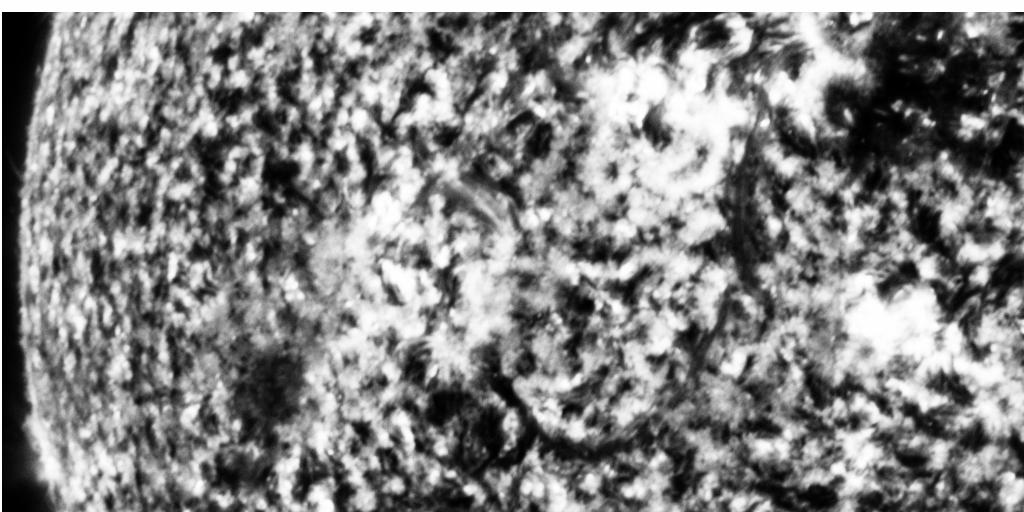
\includegraphics[width=\textwidth]{images/exp2} \\
			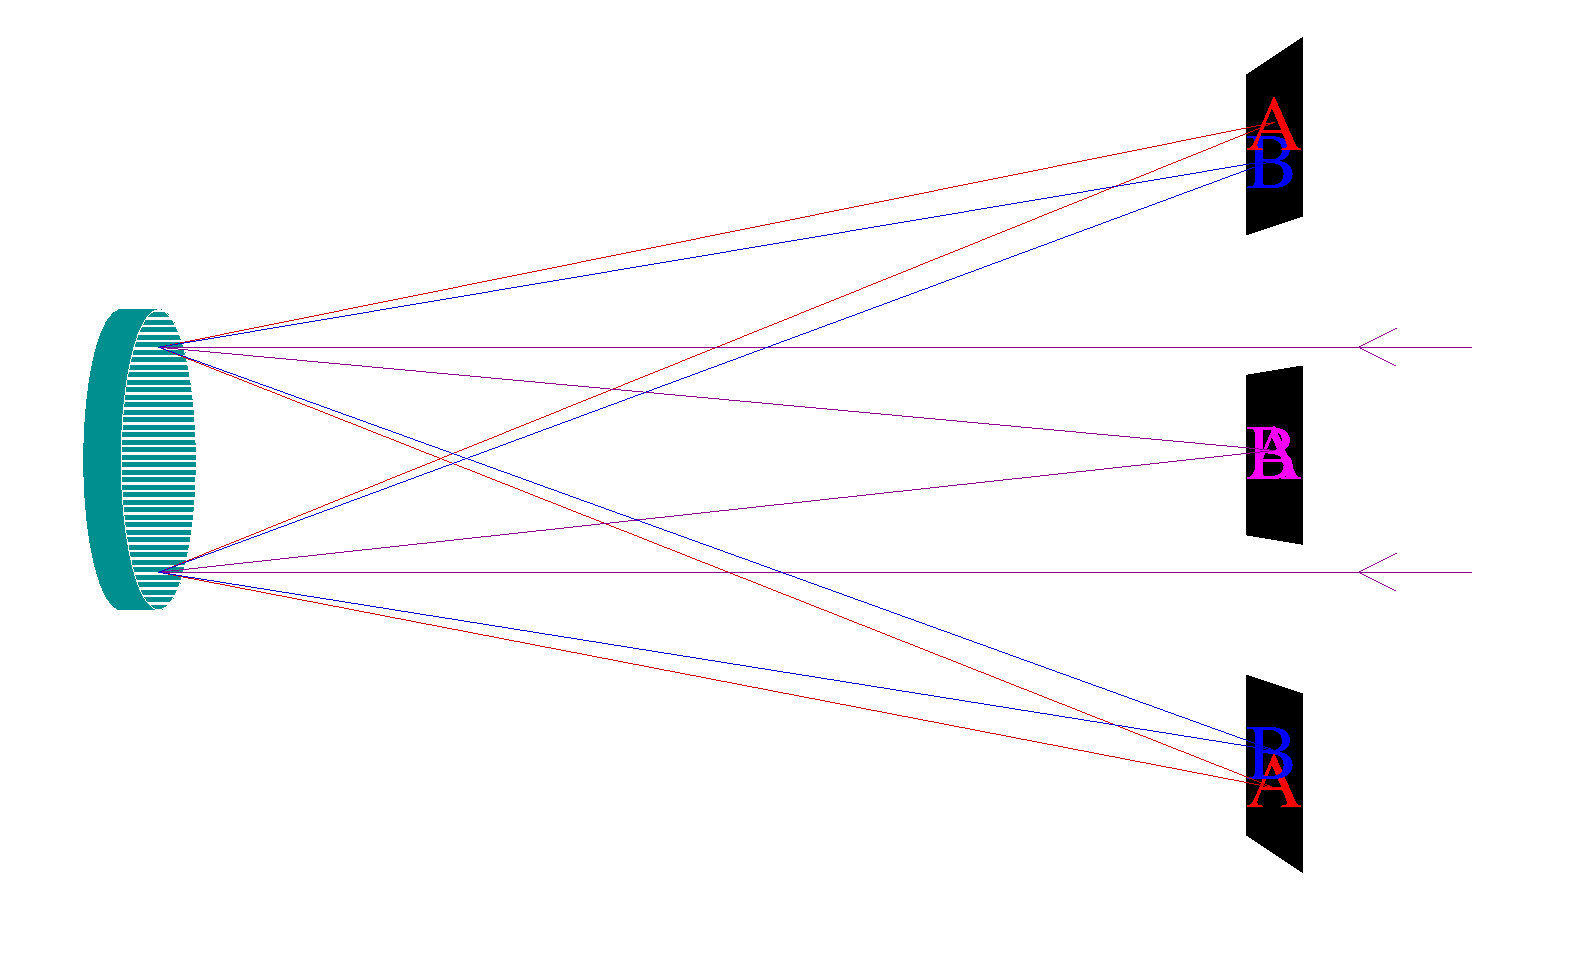
\includegraphics[width=\textwidth]{images/instrument}
		
		\end{column}%
		\end{columns}

	\end{frame}
	
	\begin{frame}
		
		\frametitle{First Launch}
		
		\begin{columns}[T] % align columns
		\begin{column}{.15\textwidth}

			\movie[width=3cm,height=7cm,poster,externalviewer]{\pgfuseimage{rocket}}{images/Launch.mp4}
			
		\end{column}%
		\hfill%
		\begin{column}{.83\textwidth}
		
			\begin{itemize}
				\item MOSES first launched on February 8th, 2006 \cite{moses}.
				\begin{itemize}
					\item Utilized a Black Brant IX sounding rocket
					\item Observed the Sun in He II 304 \AA
					\item Identified a Transition Region Explosive Event.
					\item Hercules EBX flight computer was damaged after launch. We hypothesize that this occurred upon splashdown into atmosphere.
				\end{itemize}
				\item MOSES II
				\begin{itemize}
					\item Following the first operation, the MOSES research group planned to try again with updated optics.
					\item Necessitated replacing the malfunctioning flight computer. Unfortunately the Hercules board used for the first flight is no longer available.
					\item New flight computer was to be developed to act as a drop-in replacement for the old system.
				\end{itemize}
			\end{itemize}
		
		\end{column}%
		\end{columns}
	
	\end{frame}
		
	\begin{frame}
	
		\frametitle{System Requirements}
		
				\begin{columns}[T] % align columns
				\begin{column}{.49\textwidth}
					\begin{itemize}
						\item Data characteristics
						\begin{itemize}
							\item MOSES captures the sun in three spectral orders $m=-1,0,1$.
							\item Each spectral order is captured by CCDs at $2048 \times 1024$ resolution.
								
						\end{itemize}
					\end{itemize}
					
				\end{column}%
				\hfill%
				\begin{column}{.49\textwidth}
				
					\begin{itemize}
						\item Challenges
						\begin{itemize}
							\item Short flight time, FC must be fast enough to prevent bottlenecks.
							\item Camera data is presented as 32 Mbit/s 16-bit parallel data.
						\end{itemize}
					\end{itemize}
				
				\end{column}%
				\end{columns}
		
		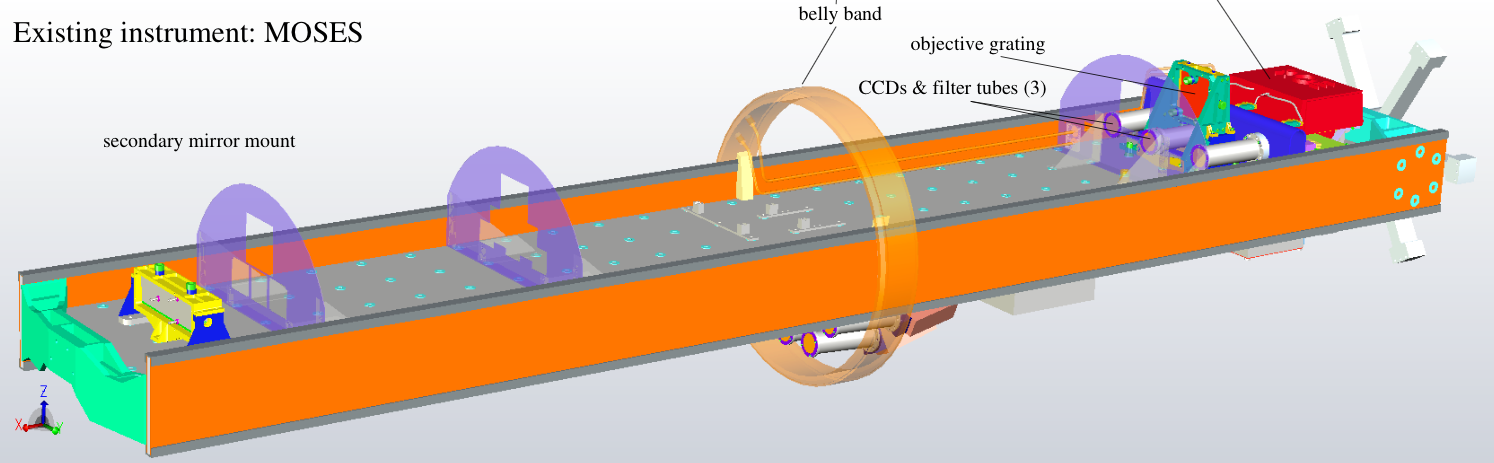
\includegraphics[width=\textwidth]{images/moses}

	\end{frame}
	
	\begin{frame}
		
		\frametitle{Hardware Overview}
		
		\begin{columns}[T] % align columns
		\begin{column}{.68\textwidth}

			\begin{itemize}
				\item Originally attempted to replace the Hercules EBX with the TS-7600 embedded system.
				\begin{itemize}
					\item Found that the FPGA implementation was too slow to keep up with the data rate.
				\end{itemize}
				\item VDX104+ Flight Computer
				\begin{itemize}
					\item Moderates communications between the ground, cameras, and FPGA.
					\item Executes flight software we developed.
				\end{itemize}
				\item Connecttech PCI104 FPGA
				\begin{itemize}
					\item Captures parallel data produced by cameras and transfers it back to VDX FC.
				\end{itemize}
					
			\end{itemize}
		
		\end{column}%
		\hfill%
		\begin{column}{.30\textwidth}

			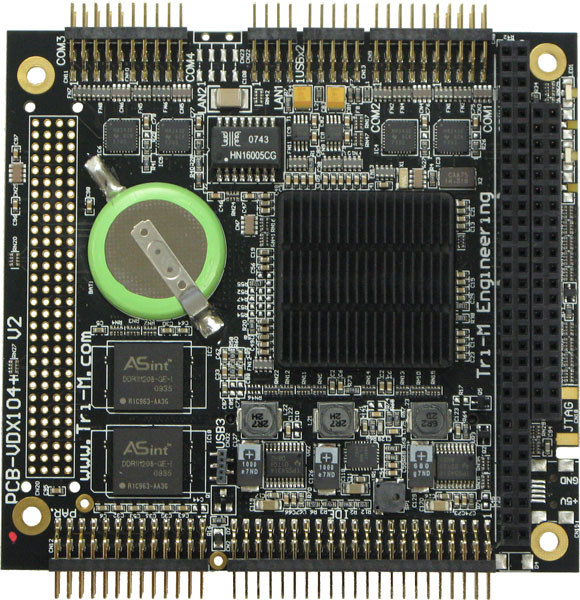
\includegraphics[width=\textwidth]{images/vdx104} \\
			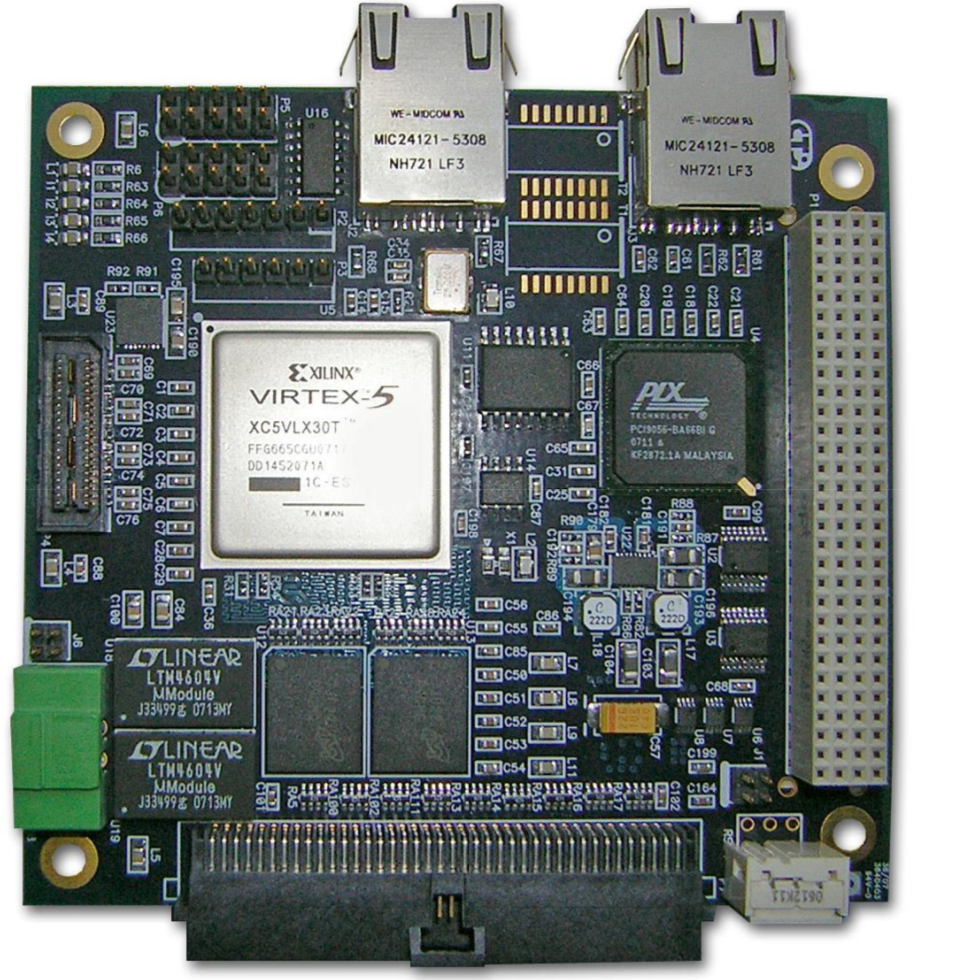
\includegraphics[width=\textwidth]{images/fpga}
					
		\end{column}%
		\end{columns}
			

	\end{frame}
	
	\begin{frame}
		
		\frametitle{Flight Software}
		
		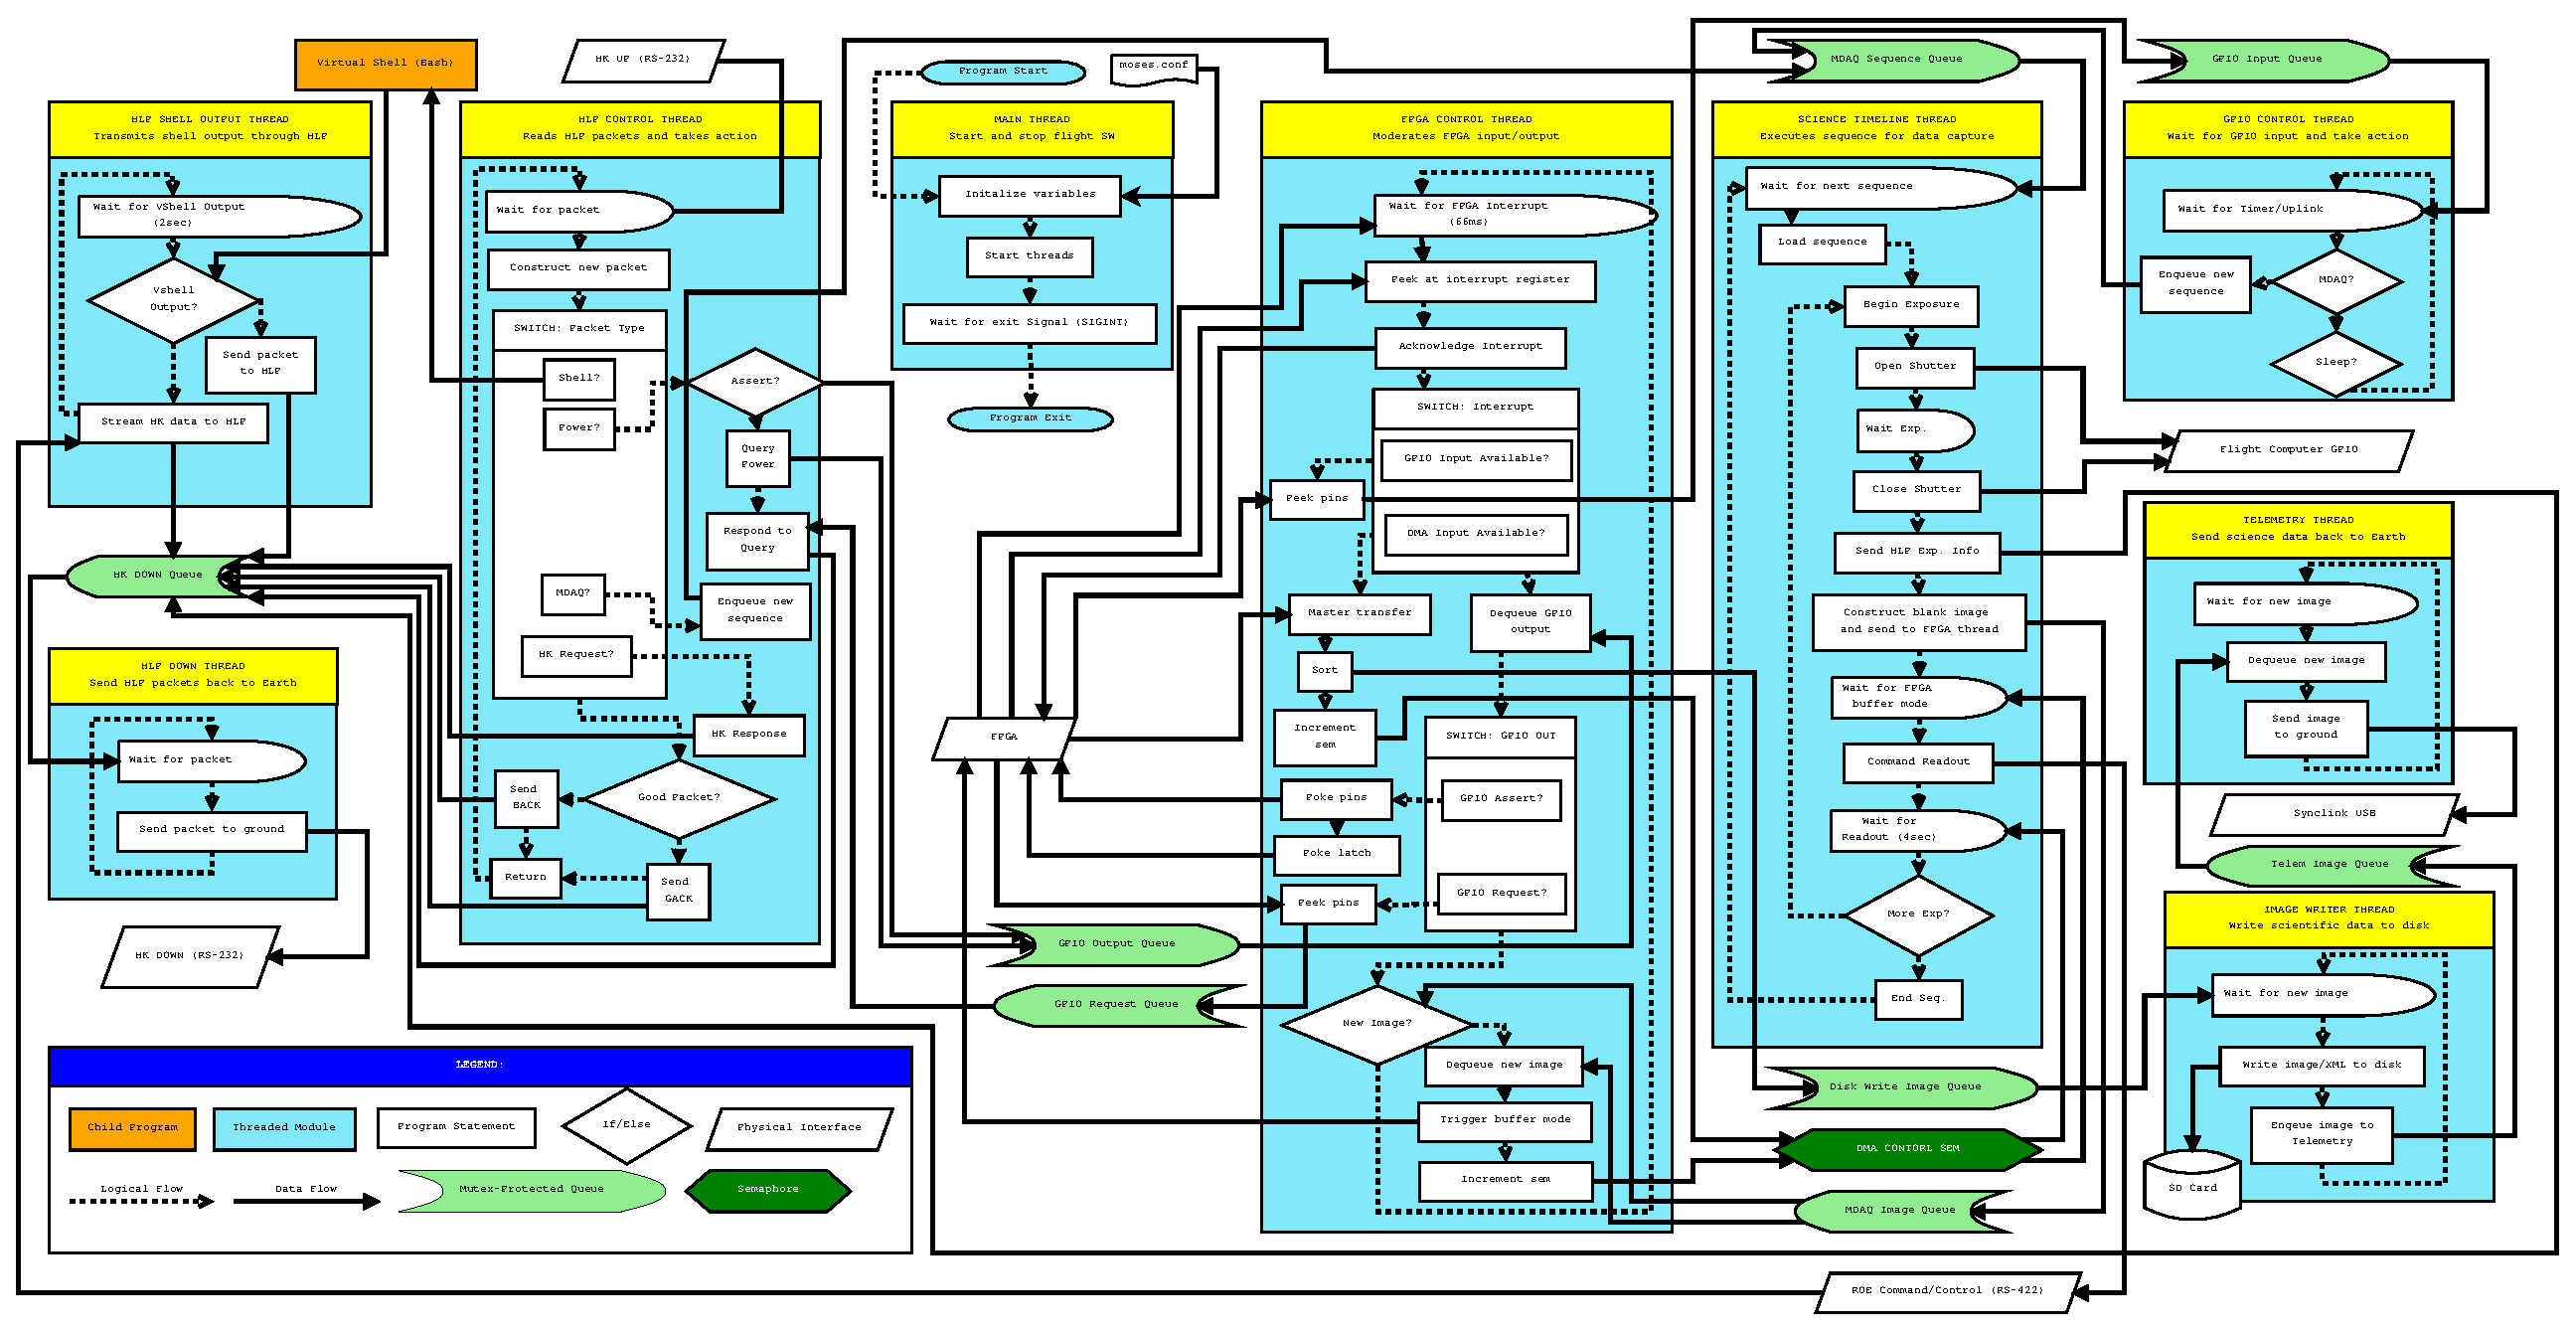
\includegraphics[width=\textwidth]{images/mfsw_block}

	\end{frame}
	
	\begin{frame}
		
		\frametitle{Ground Station Software}
		
		\begin{columns}[T] % align columns
		\begin{column}{.53\textwidth}

			 \begin{itemize}
				  	\item{Server module}
				  	\item{Client module}
				  	\item{Grounded communication}
				  	\begin{itemize}
				  		\item{Serial console}
				  		\item{Ethernet}
				  	\end{itemize}
				  	\item{In-flight communication}
					\begin{itemize}
				  		\item{Housekeeping Link Protocol (HLP)}
				  		\item{Timers}
				  		\item{High-speed telemetry}
				  	\end{itemize}
			 \end{itemize}
			
		\end{column}%
		\hfill%
		\begin{column}{.45\textwidth}

			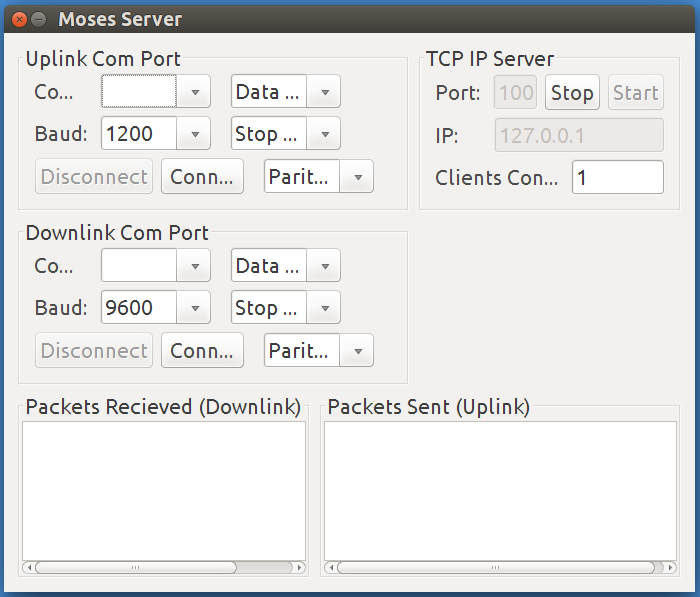
\includegraphics[width=0.7\textwidth]{server_scr} \\
			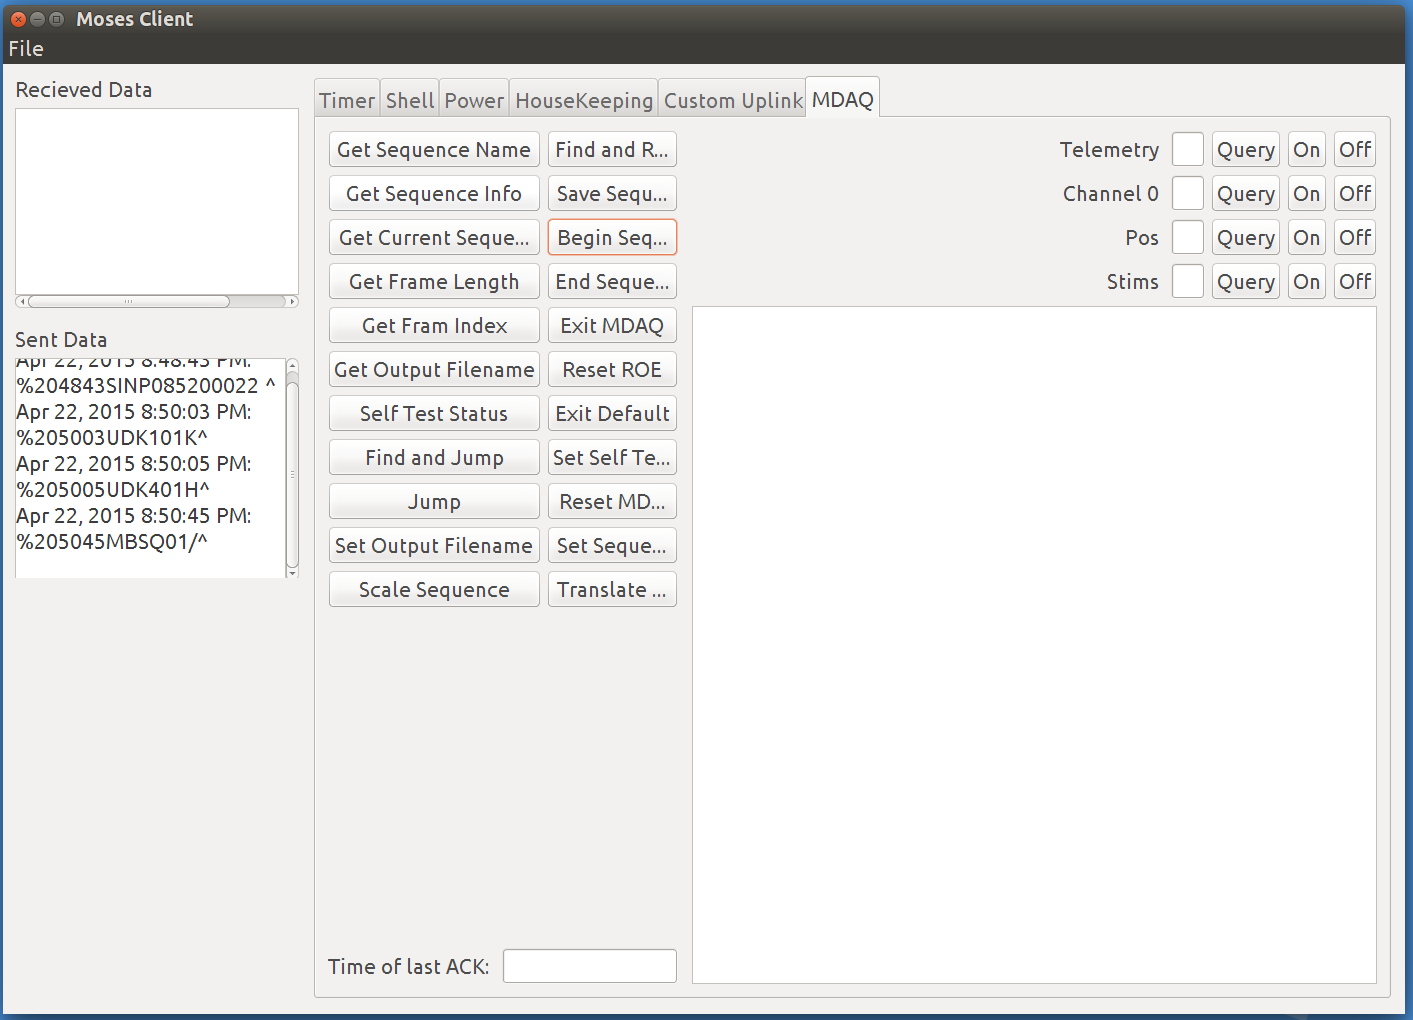
\includegraphics[width=\textwidth]{client_scr}
					
		\end{column}%
		\end{columns}

	\end{frame}
	
	\begin{frame}
		
		\frametitle{Capturing Data}
		
		\begin{columns}[T] % align columns
		\begin{column}{.49\textwidth}

			
\includegraphics[width=\textwidth]{images/selftest_plus} \\
			
\includegraphics[width=\textwidth]{images/stims_zero}
			
		\end{column}%
		\hfill%
		\begin{column}{.49\textwidth}
		
			\begin{itemize}
		  		\item STIM(S)
		  		\item ReadOut Electronics (ROE) shown to be functional
		  	\end{itemize}
		
		\end{column}%
		\end{columns}
		

	\end{frame}
	
	\begin{frame}
		
		\frametitle{Data Retrieval}
		
		\begin{columns}[T] % align columns
		\begin{column}{.49\textwidth}

			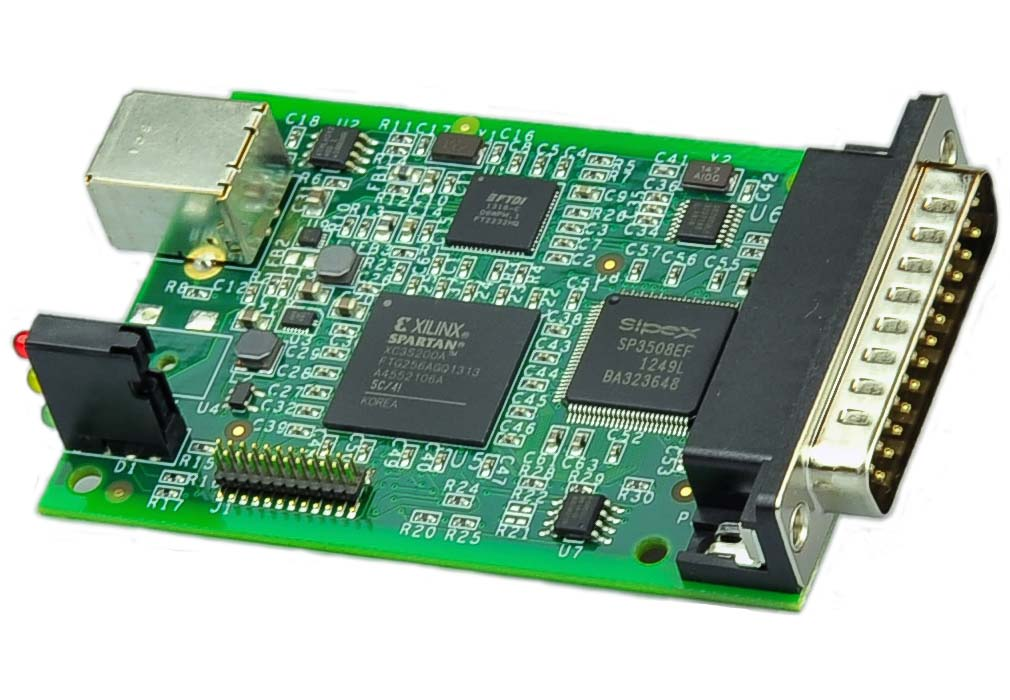
\includegraphics[width=0.5\textwidth]{images/synclink} \\
			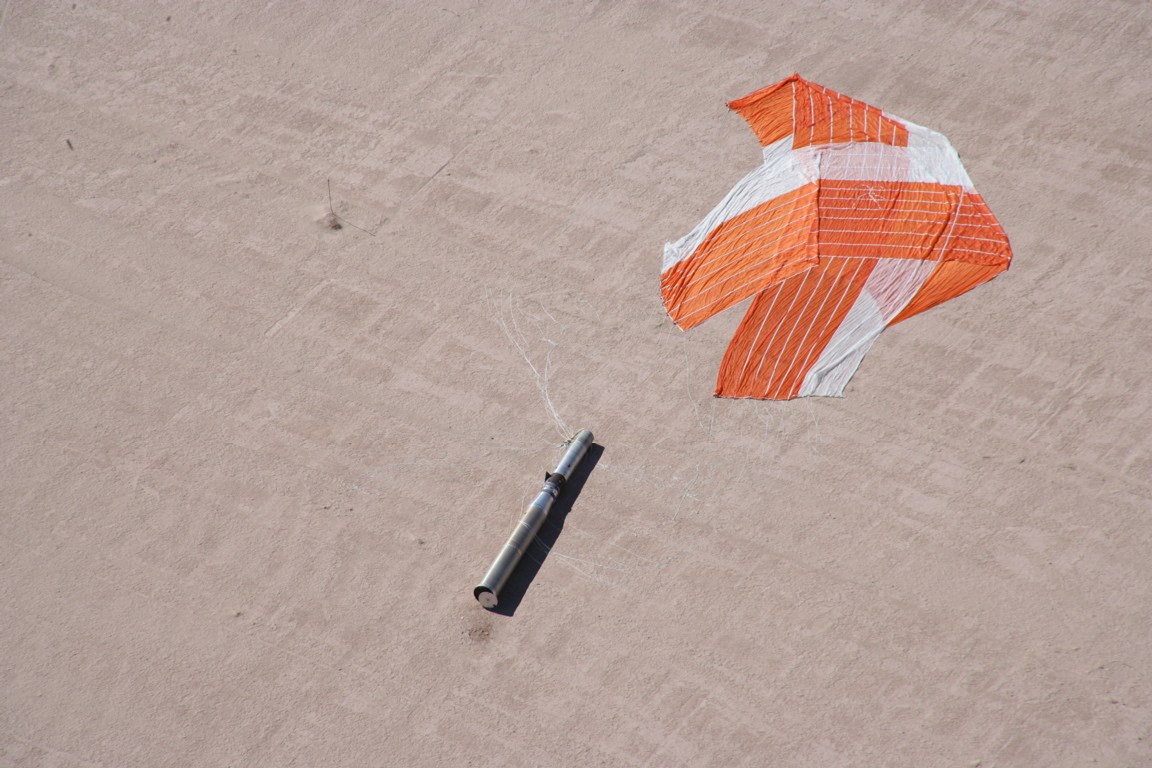
\includegraphics[width=\textwidth]{images/desert}
			
		\end{column}%
		\hfill%
		\begin{column}{.49\textwidth}

			\begin{itemize}
				\item High-Speed Telemetry
				\item Synclink implementation
				\item Pre-Mod Filter
				\item Groundstation Laptop / IDL image view
		  	\end{itemize}
					
		\end{column}%
		\end{columns}

	\end{frame}
	
	\begin{frame}
		
		\frametitle{Next Launch}
		
		\begin{columns}[T] % align columns
		\begin{column}{.49\textwidth}

			\begin{itemize}
				\item Scheduled for launch: August 17(27?)
				\item Horizontal test in progress
				\begin{itemize}
					\item Interaction/control over other payload components
				\end{itemize}
			\end{itemize}			
			
		\end{column}%
		\hfill%
		\begin{column}{.49\textwidth}

			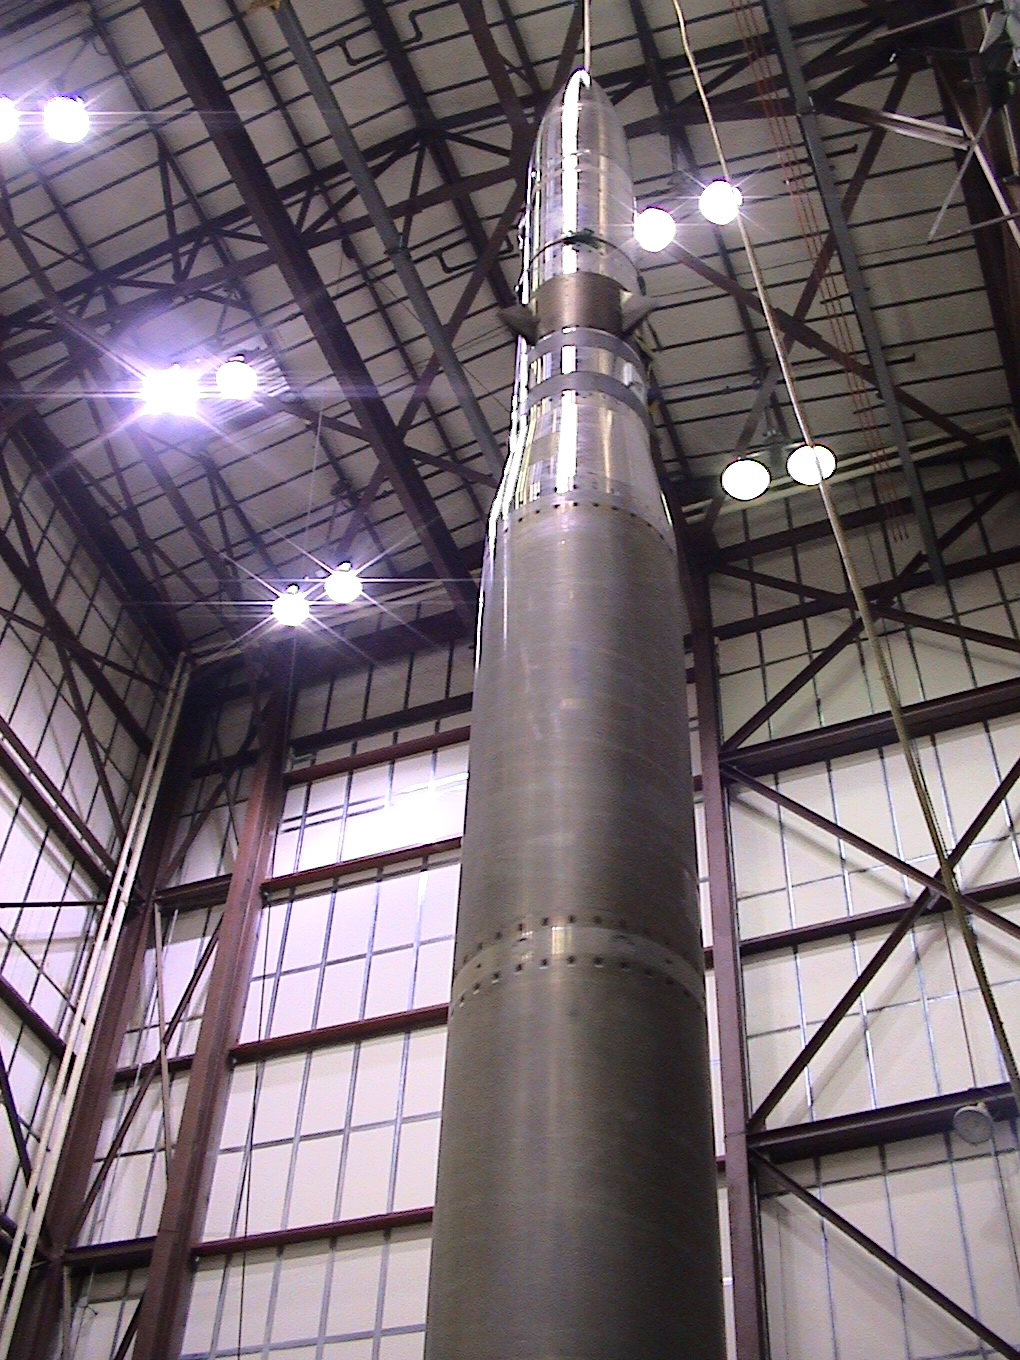
\includegraphics[width=\textwidth]{images/high}
					
		\end{column}%
		\end{columns}

	\end{frame}
	
	\begin{frame}
		\frametitle{References}
		
		\bibliographystyle{unsrt}
		\bibliography{sources}
	\end{frame}
	
\end{document}








